\documentclass[a4paper]{article}
\usepackage[spanish]{babel}
\usepackage[utf8]{inputenc}
\usepackage{charter}   % tipografia
\usepackage{graphicx}
\usepackage{courier}
%\usepackage{makeidx}
\usepackage{paralist} %itemize inline

%\usepackage{float}
\usepackage{amsmath, amsthm, amssymb}
%\usepackage{amsfonts}
%\usepackage{sectsty}
%\usepackage{charter}
%\usepackage{wrapfig}
%\usepackage{listings}
%\lstset{language=C}

\usepackage{color} % para snipets de codigo coloreados
\usepackage{fancybox}  % para el sbox de los snipets de codigo

\definecolor{litegrey}{gray}{0.94}

% \newenvironment{sidebar}{%
% 	\begin{Sbox}\begin{minipage}{.85\textwidth}}%
% 	{\end{minipage}\end{Sbox}%
% 		\begin{center}\setlength{\fboxsep}{6pt}%
% 		\shadowbox{\TheSbox}\end{center}}
% \newenvironment{warning}{%
% 	\begin{Sbox}\begin{minipage}{.85\textwidth}\sffamily\lite\small\RaggedRight}%
% 	{\end{minipage}\end{Sbox}%
% 		\begin{center}\setlength{\fboxsep}{6pt}%
% 		\colorbox{litegrey}{\TheSbox}\end{center}}

\newenvironment{codesnippet}{%
	\begin{Sbox}\begin{minipage}{\textwidth}\sffamily\small}%
	{\end{minipage}\end{Sbox}%
		\begin{center}%
		\vspace{-0.4cm}\colorbox{litegrey}{\TheSbox}\end{center}\vspace{0.3cm}}



\usepackage{fancyhdr}
\pagestyle{fancy}

%\renewcommand{\chaptermark}[1]{\markboth{#1}{}}
\renewcommand{\sectionmark}[1]{\markright{\thesection\ - #1}}

\fancyhf{}

\fancyhead[LO]{Sección \rightmark} % \thesection\ 
\fancyfoot[LO]{\small{Martín Fosco, Javier Minces, Cristian Chibana}}
\fancyfoot[RO]{\thepage}
\renewcommand{\headrulewidth}{0.5pt}
\renewcommand{\footrulewidth}{0.5pt}
\setlength{\hoffset}{-0.8in}
\setlength{\textwidth}{16cm}
%\setlength{\hoffset}{-1.1cm}
%\setlength{\textwidth}{16cm}
\setlength{\headsep}{0.5cm}
\setlength{\textheight}{25cm}
\setlength{\voffset}{-0.7in}
\setlength{\headwidth}{\textwidth}
\setlength{\headheight}{13.1pt}

\renewcommand{\baselinestretch}{1.1}  % line spacing
% \setcounter{secnumdepth}{2}
\usepackage{underscore}
\usepackage{caratula}
\usepackage{url}


\begin{document}


\thispagestyle{empty}
\materia{Métodos Numéricos}
\submateria{Segundo Cuatrimestre de 2014}
\titulo{Trabajo Práctico 3}
\subtitulo{Develando la mentira de los megap\'{i}xeles}
\integrante{Fosco, Martin Esteban}{449/13}{mfosco65@gmail.com}
\integrante{Minces Müller, Javier Nicolás}{231/13}{javijavi1994@gmail.com}
\integrante{Chibana, Christian Ezequiel}{586/13}{christian.chiba93@gmail.com}

\maketitle
\newpage

\thispagestyle{empty}
\vfill
\begin{abstract}
En este trabajo se analizan cuatro métodos para obtener una imagen a color a partir de su $Bayer Array$. Se compara su tiempo de ejecución, así como la calidad de las imágenes obtenidas.
\end{abstract}

\thispagestyle{empty}
\vspace{3cm}
\tableofcontents
\newpage


%\normalsize

\section{Introducci\'{o}n Te\'{o}rica}
\label{sec:intro}

%Mostrar un bayer array, + un ejemplo de imagen bayerizada

%Explicación intuitiva de los métodos:
%El bilineal agarra el promedio de los 4 verdes de alrededor, porque el punto medio en una interpolación lineal es el promedio
%El direccional usa splines para completar una fila o una columna. Además, toma el gradiente (fórmula del gradiente) proque cuanto más cambio de color, más probabilidad de borde, y entonces lo que hay del otro lado importa menos

En este Trabajo Práctico se busca resolver el problema de \textit{Demosaicing} aplicado a un Bayer Array por medio de distintas alternativas (implementando distintos algoritmos capaces de resolverlo). Hecho esto se busca contrastar los resultados obtenidos por medio del método que ofrece una medición de calidad conocido como \textit{peak signal to noise ratio}. \\ \\

El Bayer Array es la forma más difundida de tomar imágenes en cámaras digitales. Dado el costo de poder detectar los tres canales primarios de color en cada pixel, se utiliza esta distribución de fotodiodos sensibles a cada canal:

\begin{figure}[htbp]
\centering
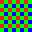
\includegraphics[width=120pt]{img/BA.png}
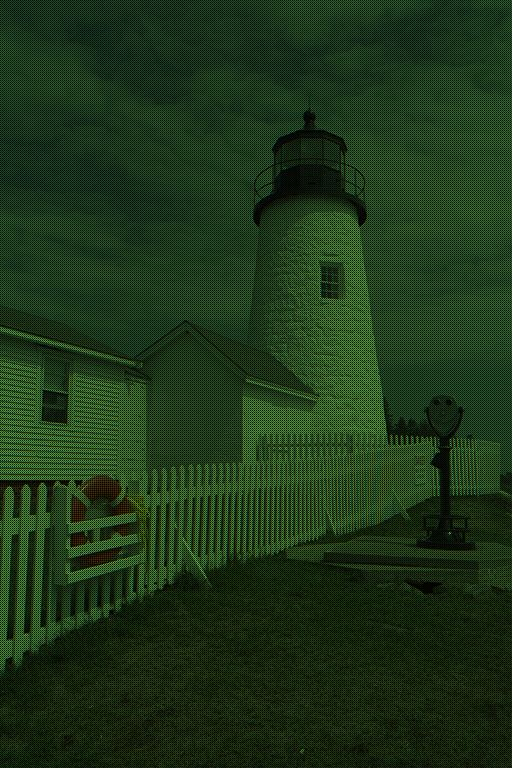
\includegraphics[width=120pt]{img/img8b.png}
\caption{Bayer Array e imagen con esta distribución}
\end{figure}

Las imagen se toman como matrices de píxeles. Cada píxel tiene un canal rojo, uno verde y uno azul, cuyo valor está siempre entre 0 y 255. En el Bayer Array hay el doble de píxeles verdes que rojos y azules, porque este es el color al que el ojo humano es más sensible.

En este trabajo se tomaron imágenes a color y se generó artificialmente su Bayer Array utilizando MatLab. De esta forma, se pueden comparar los resultados obtenidos con la imagen original%Esto probablemente vaya en otra parte

Los métodos implementados son:\\

\begin{description}

\item[Vecino Más Cercano]: Este algoritmo sigue una idea muy simple, la de tomar los valores de colores que se busca definir en una posición de su píxel vecino \footnote{Se considera que una posición es vecina a otra si se encuentran ubicadas de forma que alguno de sus extremos se tocan (puede estar en diagonal, horizontal o vertical).}que tiene ese color definido.\\

\item[Interpolación Bilineal]: La Bilineal es más compleja que \textit{Vecino Más Cercano}; si bien para determinar un pixel se recurre también a aquellos vecinos a él. Como su nombre lo dice, recurre a la interpolación entre los vecinos (promedio).\\ %Saqué el considerablemente porque la verdad que es simple

\item[Interpolación por Direcciones]: Aún más complejo que los dos anteriores es este método, que recurre a usar la interpolación con splines cúbicos sobre los vectores que cuentan con el punto a determinar en dos direcciones (vertical y horizontal) y luego incorpora los valores obtenidos dándole mayor peso a aquel al que corresponda el gradiente menor. Este se debe a que un valor absoluto alto de gradiente implica una gran variación de color, es decir, un borde.

\item[Algoritmo de Malvar, He y Cutler]: Este método presenta una mejoría en comparación con los anteriormente presentados: toma el método de \textit{Interpolación Bilineal} como base para desarrollar un método que, a la hora de decidir como incorporar los valores obtenidos de la interpolación, procede a analizar los valores de todos los canales de los pixeles cercanos y el propio para determinar los cambios de luminosidad.\\

\end{description}


\newpage

\section{Desarrollo}
\label{sec:desarrollo}
%Deben explicarse los métodos numéricos que utilizaron y su aplicación al problema concreto involucrado en el trabajo práctico. Se deben mencionar los pasos que siguieron para implementar los algoritmos, las dificultades que fueron encontrando y la descripción de cómo las fueron resolviendo. Explicar también cómo fueron planteadas y realizadas las mediciones experimentales. Los ensayos fallidos, hipótesis y conjeturas equivocadas, experimentos y métodos malogrados deben figurar en esta sección, con una breve explicación de los motivos de estas fallas (en caso de ser conocidas).

Se utilizaron los métodos listados a continuación para determinar el valor verde de los píxeles originalmente rojos y azules, mientras que se rellenaron los valores rojos y azules usando Interpolación Bilineal. Esta decisión fue tomada debido a que al ser el verde el color que más presente se hace en los Bayer Arrays y, en consecuencia, el que más impacto hace en la imagen. Es por esto que se consideró que era suficiente con comparar los métodos según los valores verdes tomados.\\ \\ %Perdón Fosqui, pero quedo mucho mejor así, sin Nota:
\textbf{Nota:} Se define:
\begin{itemize}
\item $M$ como la matriz obtenida a partir de la imagen
\item $M_v(i,j)$ el valor del canal verde en $M_(ij)$

\item $n$ como el tamaño total de la matriz.
\end{itemize}

\subsection {Vecino más cercano}
La implementación del método es muy directa, ya que la idea detrás de éste es muy simple: cada color tiene al menos un vecino de cada uno de los otros colores, ya sea en un pixel adyacente o en diagonal.\\

\begin{itemize}
\item Para determinar el valor verde en los píxeles rojos se tomó el valor verde con el que contaba el píxel en la fila inmediatamente superior a este:\\
$M_{v}(i,j) = M_{v}(i-1,j)$\\

\item Para determinar el valor verde en los píxeles azules se tomó el valor verde con el que contaba el píxel en la columna a la izquierda de este.\\
$M_{v}(i,j) = M_{v}(i,j-1)$\\

\end{itemize}

\begin{figure}[htbp]
\centering
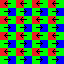
\includegraphics[width=128pt]{img/BA0.png}       %vec + cerc
\caption{Vecino Más Cercano}
\end{figure}

\subsection {Interpolación Bilineal}

Para determinar el valor de un color de un píxel con este método se calcula la interpolación lineal entre los vecinos superiores más cercanos con respecto a la fila en la que se encuentra el vector, luego la de los vecinos inferiores  más cercanos y luego se interpola estos dos valores obtenidos; este último valor es el que se define como el color del píxel a rellenar.\\
Por ejemplo, para determinar el valor verde del píxel en la fila $i$, columna $j$ :\\ \\

\noindent $InterpSup(i,j)= $\begin{Large} $\frac{M_{v}(i-1,j+1) + M_{v}(i-1,j-1)}{2}$\end{Large}\\ \\
$InterpInf(i,j)= $\begin{Large} $\frac{M_{v}(i+1,j+1) + M_{v}(i+1,j-1)}{2}$ \end{Large}\\ \\

$ M_{v}(i,j) = InterpSup(i,j) + InterInf(i,j)$\\ \\

Esto es lo mismo que:\\ 
$ M_{v}(i,j) =$\begin{Large} $\frac{M_{v}(i-1,j+1) + M_{v}(i-1,j-1) + M_{v}(i+1,j+1) + M_{v}(i+1,j-1)}{4}$ \end{Large}\\ \\

Se hace evidente al ver esta última expresión que el método se trata de hallar el promedio de los vecinos al píxel a determinar. En consecuencia, uno de los posibles problemas que se pueden encontrar al momento de implementar esta clase de algoritmos no se presenta aquí, en otras palabras, no es necesario tomar precauciones para saturar los píxeles debido a que no hay forma de que el valor resultante de un promedio sea mayor que el máximo de estos valores.

\begin{figure}[htbp]
\centering
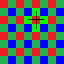
\includegraphics[width=128pt]{img/BA1.png}       %vec + cerc
\caption{Interpolación bilineal}
\end{figure}


\subsection {Interpolación direccional}
Este método consiste en aproximar el valor de cada punto mediante el uso de splines cúbicos. Se aproxima este valor con diferentes direcciones, que luego se balancean con el uso del gradiente.\\
%Subsubsection??
Un spline es una función $S(x)$, definido por partes, que interpola a una función $f(x)$ en una cantidad $n$ de puntos. Cada una de las partes de la función es un polinomio $S_j(x)$, tal que si $gr(S_j(x))=g$, $S_j\in C^{g-1} \forall j/0<j<n$ 
En el caso de los splines cúbicos, que son los más usados, tienen la forma general $a_j+b_j(x-x_j)+c_j(x-x_j)^2+d_j(x-x_j)^3$ y cumplen las siguientes condiciones:

\begin{itemize}
\item $f(x_j)=s_j(x_j) \forall j/0<j\leq n$ 
\item $S_j(x_{j+1})=S_{j+1}(x_{j+1}) \forall j/0<j<n$
\item $S'_j(x_{j+1})=S'_{j+1}(x_{j+1}) \forall j/0<j<n-1$
\item $S''_j(x_{j+1})=S''_{j+1}(x_{j+1}) \forall j/0<j<n-1$
\end{itemize}

Es decir que se tienen $4n-1$ condiciones para $4n$ incógnitas. Para generar un sistema de ecuaciones con solución única, se agrega una de las siguientes condiciones:

\begin{itemize}
\item $S''_0(x_0)=0$ y $S''_{n-1}(x_n)=0$  (spline natural o libre)
\item $S'_0(x_0)=f'(x_0)$ y $S'_{n-1}(x_n)=f'(x_n)$ (spline sujeto)
\end{itemize}

En este trabajo utilizaremos splines naturales.

Dado que $S(x_j)=a_j$ y $S(x_j)=f(x_j)$, $a_j=f(x_j) \forall j/0<j<n$. Despejando $b_j$ y $d_j$ en función de $c_j$, se obtiene que

$b_j=\frac{1}{h_j}(a_{j+1}-a_j)-\frac{h_j}{3}(2c_j)+c_{j-1})$ y

$d_j=\frac{c_{j+1}-c_j}{3h_j}$

donde $h_j=x_{j+1}-x_j$

Entonces se puede construir el siguiente sistema tridiagonal, reemplazando los valores de $b$ y $d$ y despejando $c$ en función de $a$:
\begin{center}
$\begin{bmatrix}
1   &0  &0  &   &   &   &   &   \\
h_0 &2(h_0+h_1) &h_1&0  &   &   &   &   \\
    &h_1&2(h_1+h_2) &h_2&   &   &   &   \\
    &   &h_2&2(h_2+h_3) &h_2&   &   &   \\
    &   &   &   &   &   &   &0  \\
    &   &   &   &   &h_{n-2}&2(h_{n-2}+h_{n-1})&h_{n-1}\\
    &   &   &   &   &  0&  0&1  \\
\end{bmatrix}
\cdot c = \alpha$
con $\alpha=\begin{bmatrix} 0\\ \frac{3}{h_1}(a_2-a_1)-\frac{3}{h_0}(a_1-a_0)\\ \\ \\ \\\frac{3}{h_{n-1}}(a_n-a_{n-1})-\frac{3}{h_{n-2}}(a_{n-1}-a_{n-2}) \\0 \end{bmatrix}$
\end{center}

Para resolver este sistema, se recurrió al algoritmo presentado en Burden \footnote{R. Burden y J.D.Faires, Análisis numérico, International Thomson Editors, 1998}. El algoritmo está adaptado a este caso particular en el que si, por ejemplo, si se busca interpolar la fila $i$ se conocen los puntos (0,$M_v(i,0)$), (2,$M_v(i,2)$), ... ($2j$,$M_v(i,2j)$). Es decir, $h_j=2 \forall j$.

\newcommand{\tab}{\hspace*{7mm}}
\begin{codesnippet}

interConSpline($a$):

\tab $n = size(a)$\\
\tab $\alpha$ es el vector de términos independientes.
\tab vectores auxiliares, de tamaño $n$: $l$, $\mu$, $z$\\
\\
\tab $l_0 = 1$ \\
\tab $\mu_0 = 0$ \\
\tab $Z_0 = 0$ \\
\\
\tab for i=(1:n-2)\\
\tab \tab $l_i = 8 - 2 \cdot \mu_{i-1}$ \\ %2 $\cdot$ (X_{i+1} - X_{i-1}) = 8	y	_i-1 = 1\\
\tab \tab $\mu_i = \frac{2}{l_i}$\\ %H_i = 2\\
\tab \tab $z_i = \frac{\alpha_i - 2 \cdot z_{i-1}}{l_i}$\\
\tab endfor\\
\\
\tab $l_{n-1} = 1$\\
\tab $z_{n-1} = 0$\\
\tab $c_{n-1} = 0$\\
\\
\tab for i = (n-2:0)\\
\tab \tab $c_i = z_i - \mu_i \cdot c_{i+1}$\\
\tab endfor \\
\tab return $c$
\end{codesnippet}

A partir de $c$ se calcula $b$ y $d$ con las ecuaciones presentadas anteriormente, con $h_i=2$:

$b_i = \frac{1}{2}(a_{i+1}-a_j)-\frac{2}{3}(2c_i)+c_{i-1})$\\

$d_i = \frac{c_{i+1} - c_i}{6}$ \\

En el caso de este trabajo, dado que $x-x_j=1$ para todos los valores de $x$ que buscamos calcular,
$f(x)=d_i+c_i+b_i+a_i$ con $i$ que verifica que $x_i<x<x_{i+1}$

Para balancear los resultados, se consideraron dos posibilidades:
\begin{itemize}
\item $M_v(i,j)=\frac{(255-gradH)*prH + (255-gradV)*prV)}{(255-gradH)+(255-gradV}$
\item $M_v(i,j)= \left \{\begin{array}{ll}
prH & \text{si } gradV>gradH \\ prV & \text{si } gradH \leq gradH\end{array} \right \} $

\end{itemize}
Considerando el gradiente obtenido por diferencias finitas:

$gradH=|M_{v}(i,j+1)-M_{v}(i,j-1)|$

$gradV=|M_{v}(i+1,j)-M_{v}(i-1,j)|$

Y llamando $prH$ al resultado de la interpolación por filas y $prV$ al resultado de la interpolación por columnas. Nos inclinamos por la primera posibilidad, que no descarta por completo el valor de una interpolación.

Es necesario saturar el resultado, ya que puede ser mayor a 255 o menor a 0.

\begin{figure}[htbp]
\centering
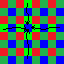
\includegraphics[width=128pt]{img/BA2.png}       %vec + cerc
\caption{Interpolación direccional}
\end{figure}

\subsection {Algoritmo de He, Malvar y Cutler}

Este algoritmo se basa en la observación de que los bordes se identifican por una diferencia mayor en los canales rojos y azules que en el canal verde.\\
Para completar un canal el algoritmo realiza su interpolación bilineal y la modifica según el gradiente de los otros canales; es decir que se utiliza a los gradientes como una suerte de $correctores$, regulado por un parámetro $\alpha$ que determina el peso de dicha corrección.

En un pixel rojo:\\ \\

$M_v(i,j)$= \begin{Large}$\frac{M_v(i,j+1)+M_v(i,j-1)+M_v(i-1,j)+M_v(i+1,j)}{4}$\end{Large} $ +\alpha \Delta_r(i,j) $\\

Con 
$\Delta_r(i,j) = M_r(i,j)-$\begin{Large}$\frac{M_r(i,j+2)+M_r(i,j-2)+M_r(i-2,j)+M_r(i+2,j)}{4} $
\end{Large}\\
En un píxel azul, la fórmula es análoga
Donde $\alpha$ representa la importancia que se le da al gradiente del color no verde. Los autores recomiendan tomar $\alpha=\frac{1}{2}$. Además, afirman que su método es mejor que todos los métodos lineales con que comparan, y tambien que algunos métodos no lineales, tanto en calidad como en tiempo de cómputo.

\begin{figure}[htbp]
\centering
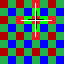
\includegraphics[width=128pt]{img/BA3.png}       %vec + cerc
\caption{Algoritmo de He, Malvar y Cutler}
\end{figure}

\subsection{Medición de Calidad: Peak Signal-to-Noise Ratio}

El criterio definido para determinar la calidad de la imagen generada se basa en compararla con la imagen original píxel a píxel. Se intenta obtener un resultado fiable y representativo de la calidad que el ojo humano detectaría en una imagen, si bien no llega a acercarse de manera pronunciada a este objetivo por ser un criterio que se basa estrictamente en la comparación numérica.\footnote{Fuente : \textit{Peak Signal-to-Noise Ratio as an Image Quality Metric}} \\
Para encontrar este valor se recurre al error cuadrático medio, de la siguiente manera:\footnote{Se excluyen los bordes de la matriz en el cálculo del PSNR debido a la dificultad que presentan a la hora de determinar el valor de sus píxeles. Esto podría cambiar drásticamente el valor obtenido por el PSNR mientras que su exclusión afecta poco la imagen generada.} \\

\begin{footnotesize}
\noindent $O=matriz\ original\\  N=nueva\ matriz$\\ \\
\end{footnotesize}
\begin{large}
$mse = \sum_{i=2}^{f-1}\sum_{j=2}^{c-1}\frac{ O_{i,j} - N_{i,j}}{(f-2) \cdot (c-2)}$\\ \\

\textit{PSNR} $= 10 \times log_{10}\left (\frac{255^2}{mse} \right )$\\ \\
\end{large}

Cuanto mayor sea el valor de PSNR obtenido para la comparación entre las imágenes, se considera que la nueva imagen generada es mejor, es decir que presenta menos ruido. Eneste trabajo se considera únicamente el PSNR sobre el canal verde, por ser el más importante para el ojo humano.

\newpage
\section{Resultados y Discusi\'{o}n}
\label{sec:res}


%Deben incluir los resultados de los experimentos, utilizando el formato más adecuados para su presentación. Deberán especificar claramente a qué experiencia corresponde cada resultado. No se incluirán aquí corridas de máquina.

%Se incluirá aquí un análisis de los resultados obtenidos en la sección anterior (se analizará su validez, coherencia, etc.). Deben analizarse como mínimo los ítems pedidos en el enunciado. No es aceptable decir que “los resultados fueron los esperados”, sin hacer clara referencia a la teoría la cual se ajustan. Además, se deben mencionar los resultados interesantes y los casos “patológicos” encontrados.

%Una vez implementados los diferentes métodos, se debe experimentar sobre los mismos todo aspecto que el grupo crea que es interesante para un algoritmo de estas características. La experimentación deberá incluir como mínimo los siguientes aspectos:
% Tiempo de computo: Medición basada en la variación de todos los parámetros que se consideren importantes.
% Calidad cuantificable: Utilización de métricas de comparación de imágenes tales como el Peak Signal-to-Noise Ratio.
% Calidad subjetiva: Identificación y caracterización de artifacts presentes en las diferentes formas de resolución.
%En todos los casos, es importante considerar que condiciones de experimentación son interesantes variar para comparar las diferentes soluciones.

%CONTAR EL CONTEXTO DE LA EXPERIMENTACIÓN Y LO QUE ESPERAMOS PARA CADA TEST.
En la experimentación se tomaron las doce imágenes dadas por la cátedra con el $Bayer Array$ ya aplicado en cada imágen.

Para la experimentación de los distintos métodos medimos las diferencias cuantificables únicamente sobre el canal verde, utilizando \textbf{Interpolación Bilineal} para definir los canales azul y rojo en los cuatro métodos para que estos canales no afecten a la medición.

Para la medición de tiempos, se utilizó la librería $ctime$de C++, sin tomar en cuenta el tiempo de carga y devolución de la matriz, y la aplicación de la \textbf{Interpolación Bilineal} para los canales azul y rojo.

En algunos de los experimentos de calidad subjetiva, mostramos los resultados solo mostrando el canal verde para que el método aplicado para el canal rojo y azul, no afecte la calidad de la imagen.

\subsection{Resultados Esperados}

\begin{itemize}
\item Para el tiempo de cómputo se esperaba que el método de \textbf{Vecino más cercano} fuera el más rápido en la ejecución ya que, para cada píxel a determinar su canal verde, solo hace un acceso a la matriz de la imagen. 

En cuanto al método mas lento en su ejecución se esperaba que fuera el de \textbf{Interpolación direccional} ya que nuestra implementación recorre la matriz imagen una vez por cada dirección utilizada para el método, es decir, recorre dos veces la matriz para determinar el canal verde con la dirección horizontal y vertical, a diferencia de los otros métodos que recorren la matriz una sola vez. Además, debe resolver un sistema de ecuaciones (aunque tridiagonal, con orden de complejidad lineal) por cada fila y columna que recorre.

\item En la calidad cuantificable de cada método, se esperaba que el de menor calidad sea el de \textbf{Vecino más cercano} ya que tiene en cuenta menos datos, a diferencia de los otros métodos; y que el de mayor calidad sea el de \textbf{Interpolación direccional} ya que al recorrer la matriz una vez por cada dirección, obtiene más información para determinar el canal verde de cada píxel. También se esperaba que el \textbf{Algoritmo de He, Malvar y Cutler} resultara mejor que la interpolación bilineal y vecino más cercano, ya que en el paper se afirma que es mejor que todos los métodos lineales con los que se comparó. 

\item En cuanto a la calidad subjetiva, se esperaba hallar más cantidad de artifacts en los métodos de menor calidad cuantificable y que al comparar los artifacts, estos sean de menor magnitud en los métodos con mayor calidad cuantificable.

\end{itemize}


\subsection{Tiempo de cómputo}

\begin{figure}[htbp]
\centering
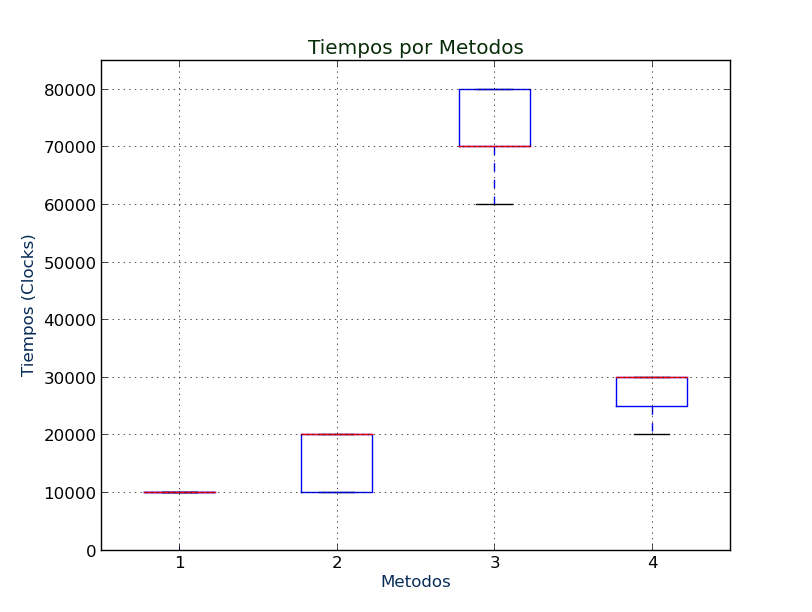
\includegraphics[width=340pt]{img/Tiempos.png}
\caption{Tiempos por método: Boxplot.\newline Se representan: percentil 9, percentil 25, mediana (línea roja), percentil 75, percentil 91, y los datos fuera de este rango como outliers.}
\end{figure}

En este gráfico ($Figura\ 2$) se puede observar que la cantidad de ciclos del método de \textbf{Direccionamiento con Splines} es por lo menos el doble que el método del \textbf{Algoritmo de He, Malvar y Cutler}, esto se debe por lo mencionado anteriormente en donde al realizar Interpolación direccional, se recorre la matriz una vez por dirección, a diferencia de los demás métodos. 

El tiempo del \textbf{Algoritmo de He, Malvar y Cutler} es mayor al método de \textbf{Interpolación Bilineal} ya que al obtener el promedio del canal verde de los píxeles verdes vecinos, el \textbf{Algoritmo de He, Malvar y Cutler} calcula el $\Delta_r$, generando cinco accesos más a la matriz.

Por último, se puede observar que el método de \textbf{Vecino más cercano} es el más rápido ya que genera un solo acceso a la matriz por píxel a determinar su canal verde, aunque suponemos que esta eficiencia temporal tendrá su contraparte en la calidad de las imágenes generadas.\newline

\newpage
\subsection{Calidad cuantificable}


%EXPLICAR PORQUÉ DIO ASÍ, Porq el paper dio mejor q el de direccionamiento splines que pusimos q esperábamos q el de splines sea mejor, porq dio muy cerquita el bilineal con splines, y ver los outliers!
En la $Figura\ 7$ se puede observar los resultados de medir el PSNR en cada método aplicada a doce imágenes distintas. Se puede observar que el método de \textbf{Vecino más cercano} da menor valor de PSNR, es decir, menor calidad cuantificable. Esto era lo esperado ya que al tomar \textbf{Vecino más cercano} en un píxel, solo toma información del canal que quiere obtener a partir de su píxel vecino.\newline
\begin{figure}[htbp]
\centering
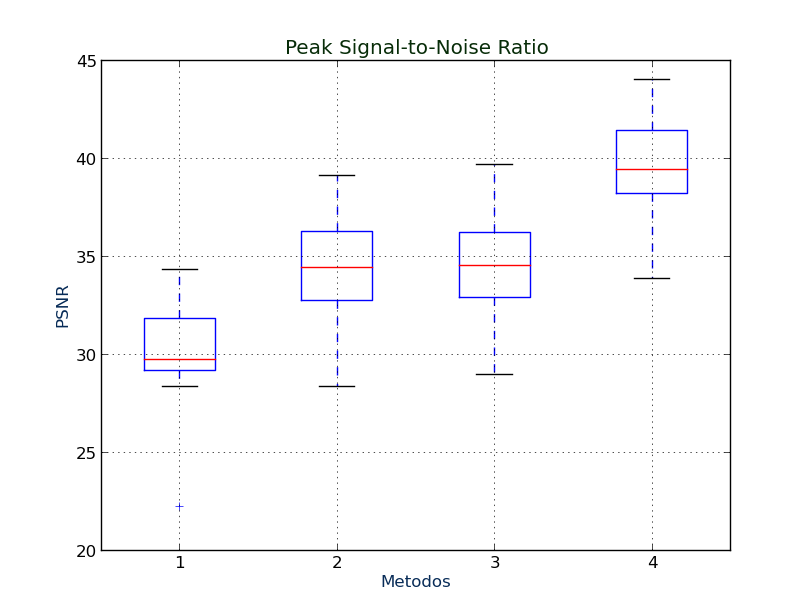
\includegraphics[width=340pt]{img/PSNR.png}
\caption{PSNR: Boxplot}
\end{figure}
El método de \textbf{Direccionamiento con Splines} resulta muy similar al método de \textbf{Interpolación Bilineal} en cuanto al PSNR. Es apenas mayor en promedio, aunque en prácticamente todas las imágenes analizadas resultó mejor. La similaridad se puede deber a que en el \textbf{Direccionamiento con Splines}, si evaluamos el spline originado por los valores de una determinada dirección en un píxel determinado buscando el canal verde, el resultado va a estar muy influenciado por los píxeles verdes adyacentes en la dirección elegida. Como las direcciones que elegimos son la vertical y la horizontal, entonces el canal verde va a estar muy influenciado por los mismos píxeles que determinan dicho canal en la \textbf{Interpolación Bilineal}, más allá del gradiente.\\

Al contrario de lo que se esperaba, se puede observar que el \textbf{Algoritmo de He, Malvar y Cutler} genera un PSNR mayor en todas las imágenes que el método de \textbf{Direccionamiento con Splines}. Analizando más profundamente cada método, creemos que el \textbf{Algoritmo de He, Malvar y Cutler} tiene mayor calidad ya que, al determinar el canal verde de un determinado píxel, utiliza información que el método de \textbf{Direccionamiento con Splines} descarta: la corrección del canal verde calculado por la \textbf{Interpolación Bilineal} utilizando el canal del píxel y sus píxeles mas cercanos del mismo canal para determinar un cambio de crominancia.\\

\newpage

\subsection{Calidad subjetiva}

Se procede a continuación a analizar los resultados obtenidos a partir de correr los algoritmos sobre distintas imágenes.


Primera Imagen:
\smallskip
%\begin{figure}[htbp]
%\centering

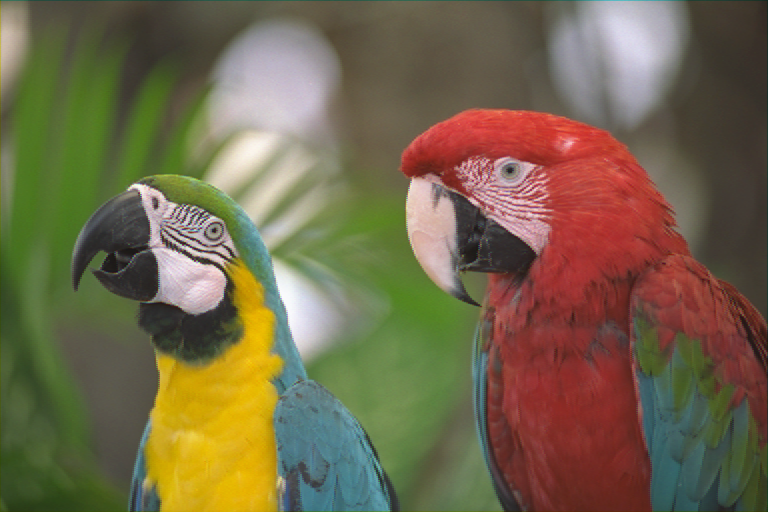
\includegraphics[width=220pt]{img/img1-0.png}       %vec + cerc
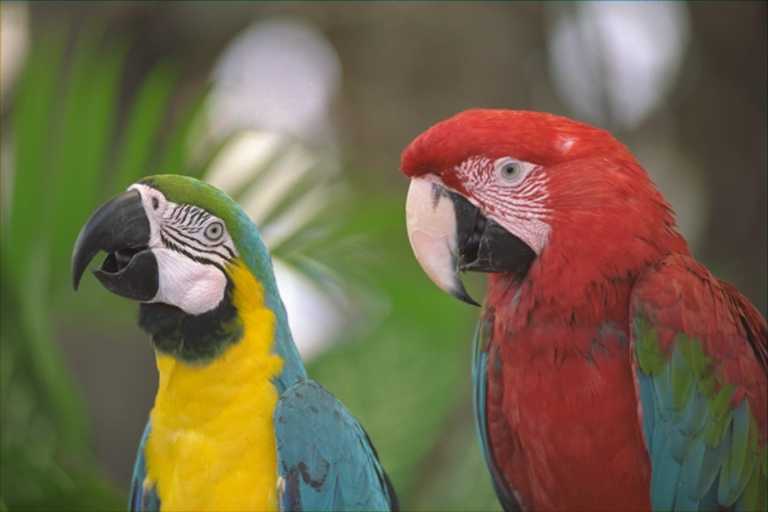
\includegraphics[width=220pt]{img/img1-1.png}       %bilin
%\end{figure}

\begin{figure}[htbp]
\centering

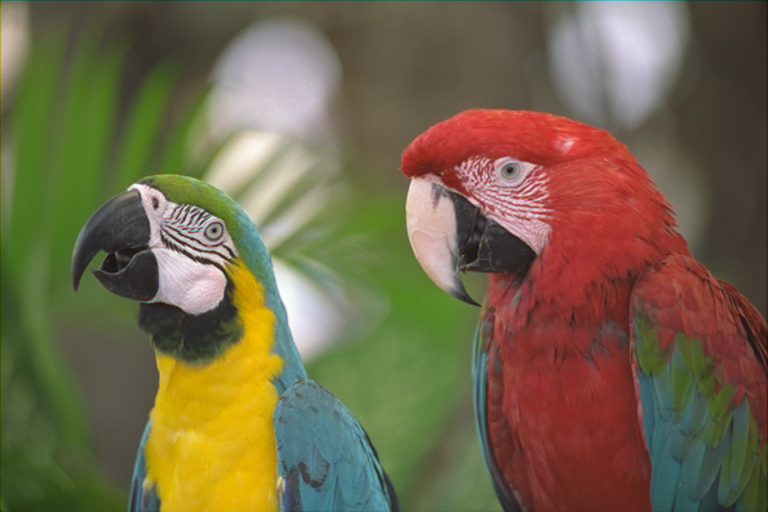
\includegraphics[width=220pt]{img/img1-2.png}       %direcc
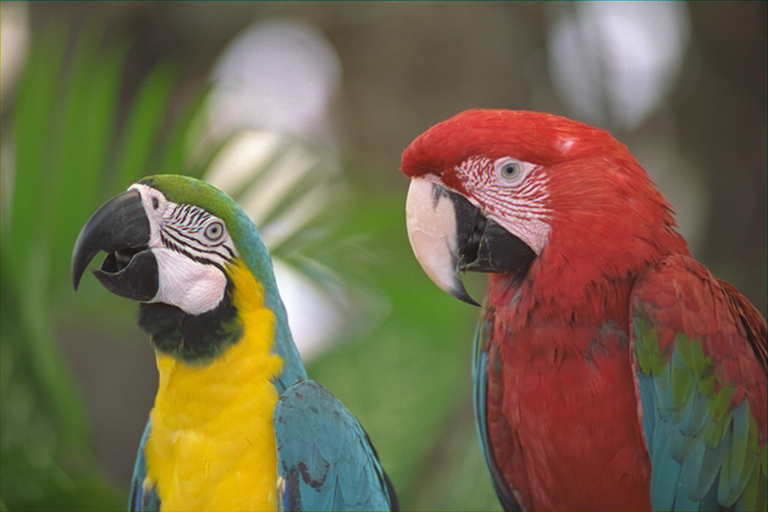
\includegraphics[width=220pt]{img/img1-3.png}       %paper

\caption{Resultados Imagen 1 - De Izquierda a Derecha: Vecino Más Cercano, Interpolación Bilineal, Interpolación por Direcciones,  Algoritmo de H, M y C}
\end{figure}

En esta primera imagen no se puede observar una gran diferencia a simple vista, si bien se nota ligeramente más borrosa la imagen resultante de aplicar \textbf{Vecino más cercano}.\\ \\ \\ \\ \\
Observando más de cerca ciertos puntos de la imagen se notan más claramente las diferencias.\\ 
Se ha omitido además aplicarle el algoritmo de Interpolación Bilineal a los rojos y azules para poder apreciar mejor la calidad de cada método:\\


\begin{figure}[h!]
\centering
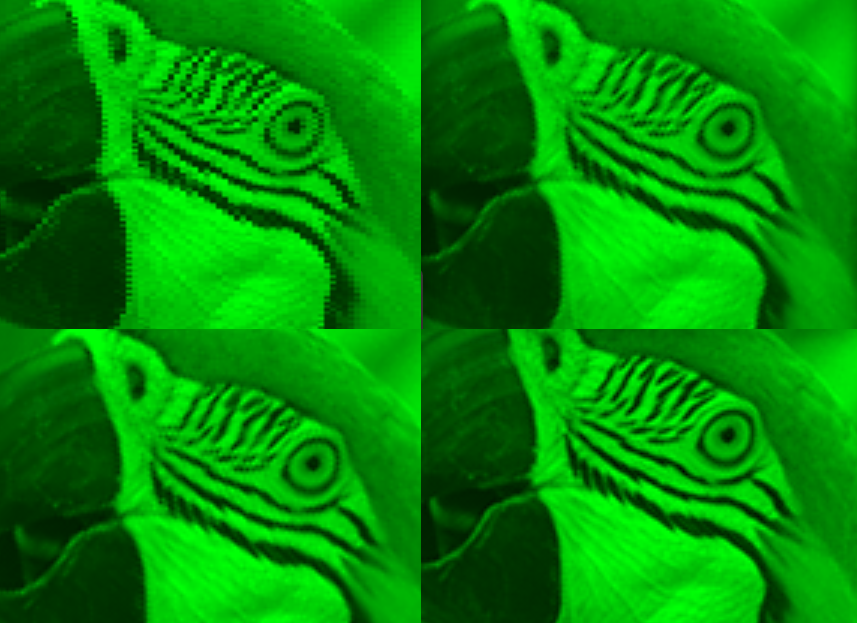
\includegraphics[width=340pt]{img/Tomo1.png}
\caption{De Izquierda a Derecha: Vecino Más Cercano, Interpolación Bilineal, Interpolación por Direcciones, Algoritmo de H, M y C}
\end{figure}

Se puede ver mejor aquí la gran diferencia que presenta el algoritmo de \textbf{Vecino más cercano}, presentando un gran grado de \textit{zippering} en los bordes, esto va en concordancia con las conjeturas hechas en el Desarrollo acerca de la calidad de este método.\\
También se puede observar que el \textbf{Algoritmo de He, Malvar y Cutler} devuelve una imagen mas definida que con los otros métodos, en particular a la hora de definir mejor las líneas arriba y a la izquierda del ojo.\newline
Por otro lado, los algoritmos que implementan interpolación bilineal y por direcciones no parecen mostrar ninguna diferencia apreciable entre sí.\newline \newline

Se puede además apreciar en otros puntos la diferencia en calidad; se puede tomar por ejemplo la parte inferior del pico del ave ubicada la izquierda en la imagen.\newline \\
\begin{center}
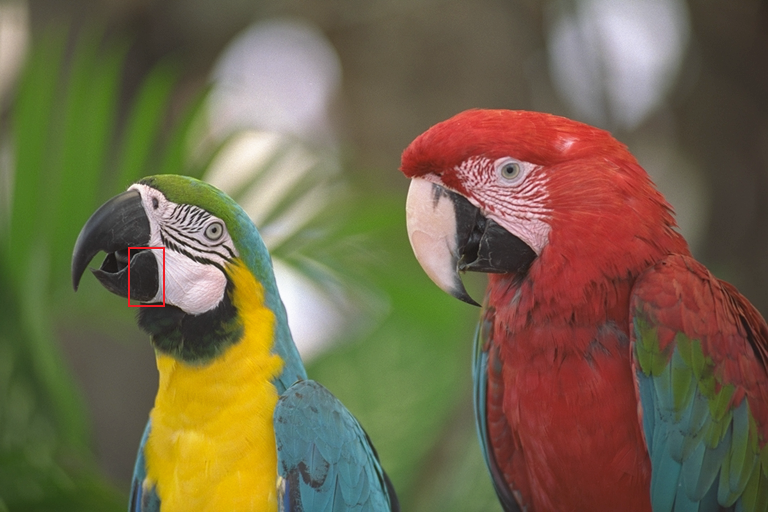
\includegraphics[width=250pt]{img/img1-con-recuadro.png}\\
\end{center}

Examinemos ahora el estado de dicha zona para los distintos métodos:\\
\begin{figure}[h!]
\centering

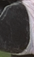
\includegraphics[width=110pt]{img/img1-recortada.png}
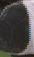
\includegraphics[width=110pt]{img/img1-0-recortada.png}
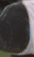
\includegraphics[width=110pt]{img/img1-1-recortada.png}\\
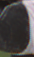
\includegraphics[width=110pt]{img/img1-2-recortada.png}
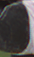
\includegraphics[width=110pt]{img/img1-3-recortada.png}
\caption{$Zippering$ en la figura 1, I-D: Original, Vec más Cercano, Int. Bilineal, Int. por Direcciones, Algoritmo de H,M,C}
\end{figure}

En esta zona en particular se ve, nuevamente, el $Zippering$ generado por \textbf{Vecino Más Cercano}.\\ \\ \\
Nuevamente, no es apreciable la diferencia que presentan los algoritmos \textbf{Interpolacion Bilineal} e \textbf{Interpolacion por Direcciones}; ambos generan resultados aceptables (si bien parece que el pico en la interpolación por Direcciones tiene una forma más definida y menos redondeada) y se acercan a la calidad del \textbf{Algoritmo de Malvar, He y Cutler}.\\
Este último, nuevamente, supera a todos los otros métodos en calidad. Esto se debe a que el del paper y el direccional funcionan mejor si el gradiente, es decir, la diferencia entre los colores del borde es mayor; y en este caso es extrema: blanco contra negro.

Es digno de mención que ninguno es capaz de eliminar por completo las líneas de colores (similares a un arcoiris) que se proyectan en la intersección entre la zona inferior y superior del pico.\\

Segunda imagen:

\begin{figure}[h!]
\centering
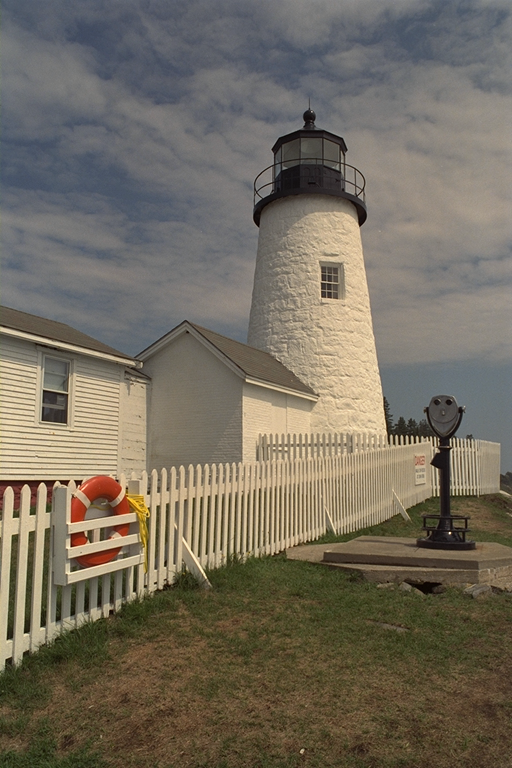
\includegraphics[width=120pt]{img/img8.png}
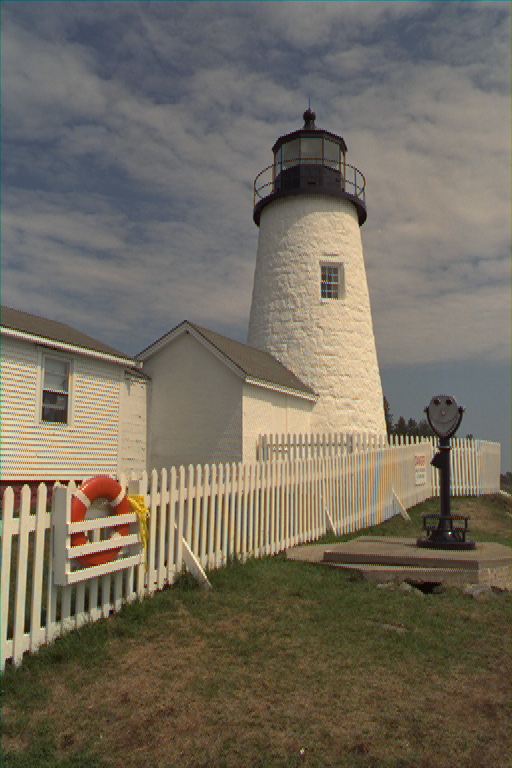
\includegraphics[width=120pt]{img/img8-0.png}
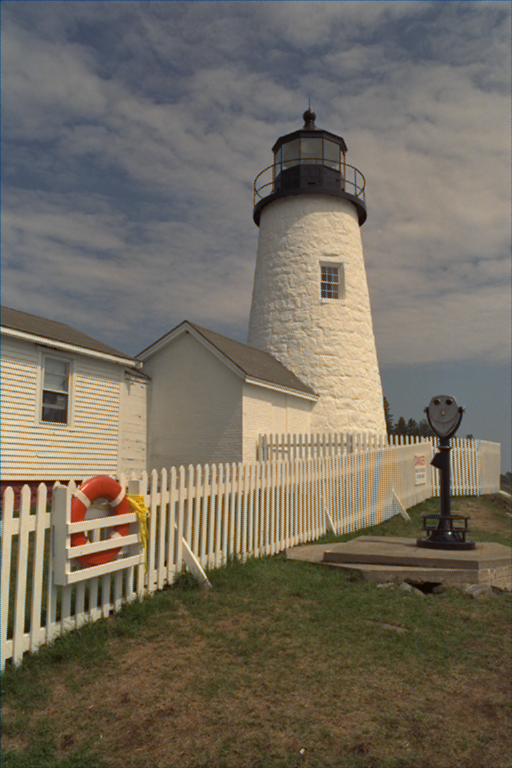
\includegraphics[width=120pt]{img/img8-1.png}
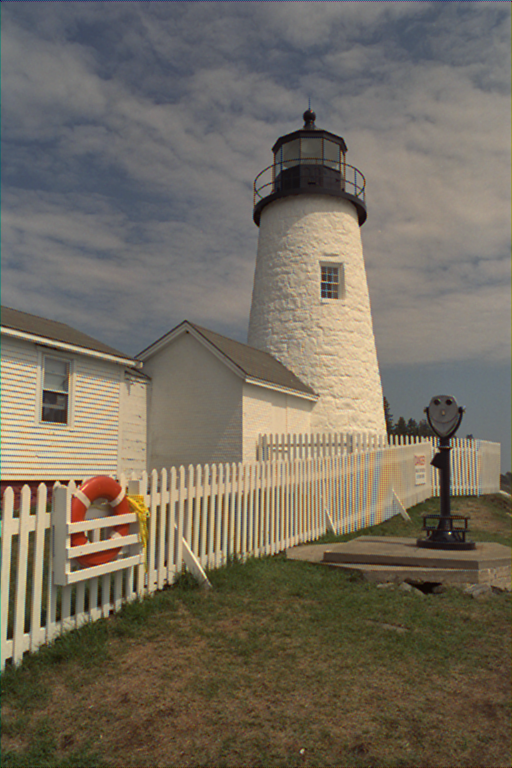
\includegraphics[width=120pt]{img/img8-2.png}
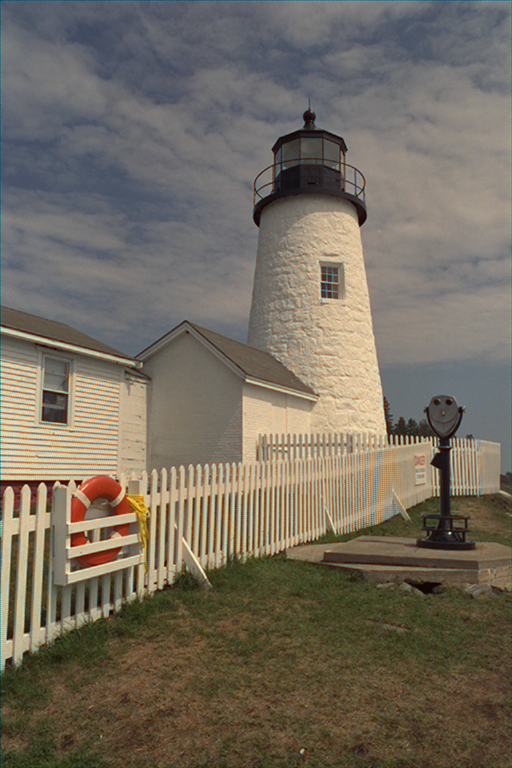
\includegraphics[width=120pt]{img/img8-3.png}
\caption{Resultados Imagen 2 - De Izquierda a Derecha: Vecino Más Cercano, Interpolación Bilineal, Interpolación por Direcciones,  Algoritmo de H, M y C}
\end{figure}

En la figura 11 se ven imágenes generadas por los distintos métodos a partir de otra imagen original. La imagen está rotada. En la valla, La sucesión de líneas verticales de distintos colores en la valla generó un patrón de Moire en todos los métodos utilizados. A diferencia de otros casos, este $artifact$ se puede notar a simple vista. De todas formas, lo analizaremos ampliando la imagen.

\begin{figure}[h!]
\centering
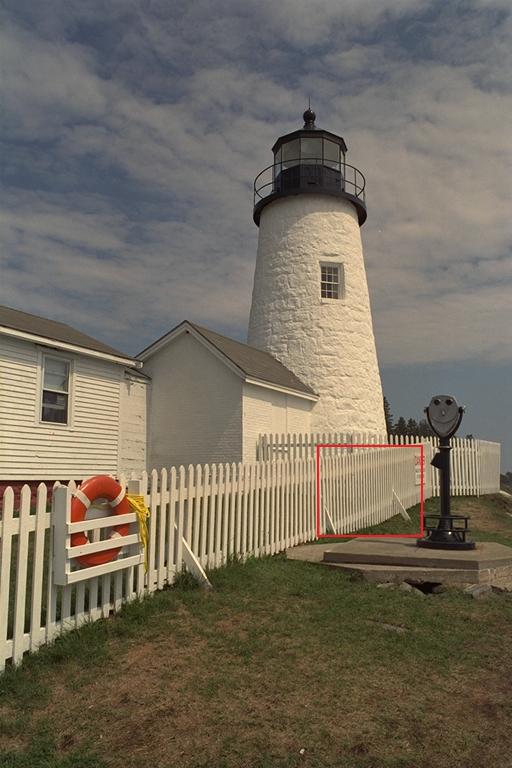
\includegraphics[width=140pt]{img/img8-con-recuadro.png}\\
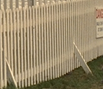
\includegraphics[width=120pt]{img/img8-recortada.png}
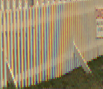
\includegraphics[width=120pt]{img/img8-0-recortada.png}
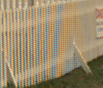
\includegraphics[width=120pt]{img/img8-1-recortada.png}\\
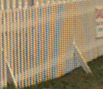
\includegraphics[width=120pt]{img/img8-2-recortada.png}
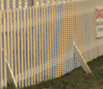
\includegraphics[width=120pt]{img/img8-3-recortada.png}
\caption{Patrones de Moire en la figura 2}
\end{figure}

En la figura 12 se pueden ver ampliaciones de una sección de la imagen original para cada método. 
Dado que este $artifact$ no se modifica con ninguno de los métodos utilizados, se pensó que podía deberse al uso de interpolación bilineal para completar los píxeles rojos y azules. Por eso, analizamos el canal verde de estas imágenes.

\begin{figure}[h!]
\centering
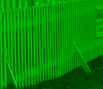
\includegraphics[width=120pt]{img/img8v-recortada.png}
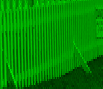
\includegraphics[width=120pt]{img/img8-0v-recortada.png}
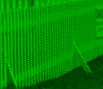
\includegraphics[width=120pt]{img/img8-1v-recortada.png}
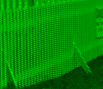
\includegraphics[width=120pt]{img/img8-2v-recortada.png}
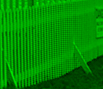
\includegraphics[width=120pt]{img/img8-3v-recortada.png}
\caption{Patrones de Moire en la figura 2: canal verde}
\end{figure}

En la figura 13 se puede contemplar que las vallas, que en la imagen original se encuentran de forma horizontal, aparecen mejor definidas en el resultado en donde se aplicó el método de \textbf{Vecino más cercano}. Al analizar este caso, comprendimos que al estar las vallas de forma horizontal y tomar al píxel más cercano en la dirección horizontal, entonces este método no toma valores innecesarios de la dirección vertical.

Esto no ocurre en los otros métodos: al tomar datos de la dirección vertical los métodos de \textbf{Interpolación Bilineal}, \textbf{Direccionamiento con Splines} y el \textbf{Algoritmo de He, Malvar y Cutler}, generan un patrón de Moire, ya que toman información que no es correcta para determinar los bordes horizontales.

\begin{figure}[h!]
\centering
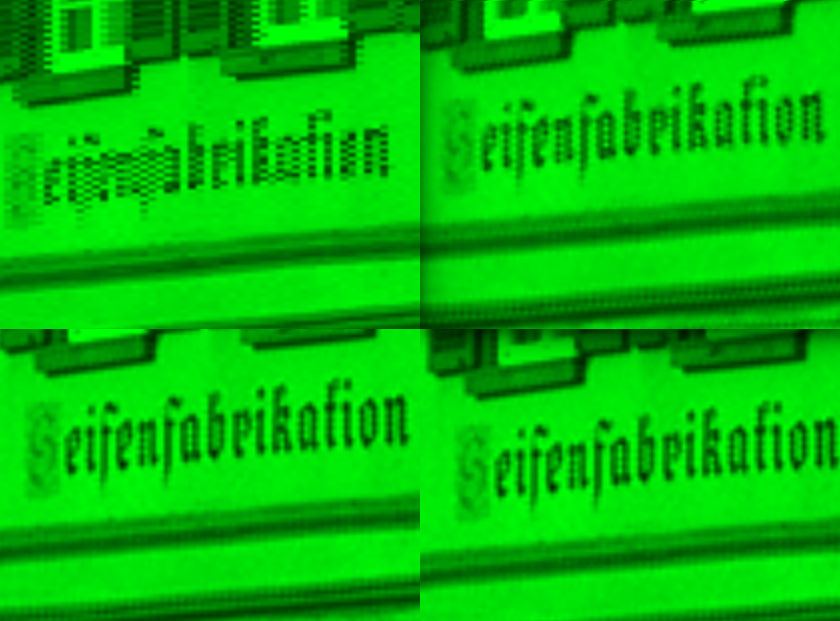
\includegraphics[width=340pt]{img/Tomo3.png}
\caption{De Izquierda a Derecha: Vecino Más Cercano, Interpolación Bilineal, Interpolación por Direcciones, Algoritmo de H, M y C: canal verde}
\end{figure}

En esta otra imagen (figura 14) se puede observar como nuestra implementación de \textbf{Vecino más cercano} presenta $zippering$ en todos los bordes verticales, pero no en los horizontales. También se observa que el método de \textbf{Direccionamiento con Splines} genera una imagen apreciablemente mejor que la imagen generada por el método de \textbf{Interpolación Bilineal}. Los cuatro métodos presentan $zippering$, pero este es mínimo en los últimos dos casos.\\

El siguiente experimento fue hecho con la intención de mostrar el comportamiento de los métodos con respecto a los bordes:\\

\begin{figure}[h!]
\centering
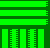
\includegraphics[width=100pt]{img/Bordes1.png}
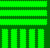
\includegraphics[width=100pt]{img/Bordes2.png}
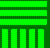
\includegraphics[width=100pt]{img/Bordes3.png}
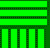
\includegraphics[width=100pt]{img/Bordes4.png}
\caption{Comportamiento frente a bordes}
\end{figure}

En la figura 15 se puede notar que el método de \textbf{Vecino más cercano} funciona mejor que los demás para bordes horizontales por la ya dicho anteriormente, y es peor que todos los demás para determinar bordes verticales. Se puede ver en la imagen de la izquierda, que algunos bordes presentan $zippering$ y otros no; esto se debe a que, en un caso, al llegar al borde, este comienza con un píxel verde que no toma valores de sus vecinos, a diferencia del otro caso en que al llegar al borde, este contiene un píxel azul (toma el canal verde del píxel de la izquierda), por lo tanto toma el canal verde mas oscuro generando así el zippering.

Comparando el método de \textbf{Interpolación Bilineal} y \textbf{Direccionamiento con Splines} se puede apreciar que el $zippering$ es más notorio en la  \textbf{Interpolación Bilineal}, esto se debe a que este método no identifica bordes, por lo tanto toma la misma cantidad de información para cada píxel. El \textbf{Direccionamiento con Splines} en cambio reconoce en los bordes, que dirección tiene menor variación de cambios, por lo tanto, el $zippering$ es menos notorio.

En el caso del \textbf{algoritmo de He, Malvar y Cutler}, reconoció los bordes, generando líneas perfectamente rectas, pero también puntos negros en la zona verde. Esto se puede deber a que los altos valores de rojo y azul en la zona blanca modifican puntos a dos píxeles de distancia.

\newpage

\section{Conclusiones}
\label{sec:conclusiones}


%Vecino más cercano no sirve de nada. Lo que sí, es rápido, así que por ahí teniendo el cuenta el tamaño de la pantallita de las cámaras digitales, es útil para mostrar la foto ni bien la sacás como pasa en muchas cámaras (wow, so fruta, much bla bla) Mentira, hubo casos en qeu reduce artifacts, considerando que por nuestra implementación las líneas horizontales quedan mejor que las verticales.
Para concluir, se pueden tomar unas apreciaciones generales acerca de los 4 métodos implementados y probados en este Trabajo Práctico:\\ \\

En el método de \textbf{Vecino Más Cercano} son observables algunas ventajas, tales como su alta eficiencia temporal (ya que no requiere procesar de ninguna manera los valores a definir en los píxeles) y la aún más notable simpleza para implementarlo.\\
Por otro lado, sin embargo, son apreciables las aún más grandes desventajas que presenta este método:\\
\begin{itemize}

\item Cuenta con una calidad altamente criticable, completamente por debajo del nivel que presentan los demás métodos.

\item Es el peor a la hora de ocultar los \textit{artifacts} presentes en distintas áreas.

\item Genera $zippering$ en los bordes que tienen sentido contrario a la selección del vecino mas cercano.

\end{itemize}

En el método de \textbf{Interpolación Bilineal} se presenta una muy buena relación entre eficiencia temporal y calidad.%Si alguien quiere chamullar mas acà mejor

En el método de \textbf{Interpolación Direccional} se pueden tomar otras direcciones, además de la vertical y la horizontal. Si no se hace eso, no produce mejoras apreciables con respecto a la \textbf{Interpolación Bilineal} (10 de 12 casos la Interpolación Direccional presentó mayor PSNR que la Interpolación Bilineal), con un costo temporal mayor.
De todas formas, el tiempo de ejecución es de décimas de segundo, por lo que las diferencias no son apreciables para imágenes de este tamaño. %a esta escala. Por ahí con imágenes más grandes, como una de stanford de 2 millones de pixeles por 2 millones de pixeles...

El \textbf{Algoritmo de He, Malvar y Cutler} resultó el mejor de los cuatro: en todas las imágenes obtuvo el mejor PSNR, con un costo temporal en la escala del método de \textbf{Interpolación Bilineal}. Esto cumple con lo afirmado en el paper. El criterio propuesto por este método, sin embargo, es aplicable a cualquier otro, por lo que pensamos que una posible mejora a intentar podría ser aplicar la modificación según $\delta_r$ dicho algoritmo al \textbf{Direccionamiento con Splines}, aunque esto aumentaría el tiempo de ejecución. Otra posible mejora a experimentar podría ser tomar para calcular la variación de la crominancia en un píxel de un canal determinado, además de los píxeles en sentido vertical y horizontal, los  píxeles del mismo canal en las diagonales: \\ 

\begin{figure}[htbp]
\centering
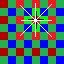
\includegraphics[width=100pt]{img/BA3Tomo.png}
\caption{Modificación propuesta}
\end{figure}


Dada la la alta varianza que presentaban los resultados del PSNR, se puede concluir que el método $objetivo$ escogido para asesorar la calidad de los algoritmos de forma cuantificable no es muy confiable a la hora de comparar métodos. En consecuencia es necesario tomar muchas muestras distintas para poder obtener una medición en la que poder apoyarse para sacar observaciones concluyentes.\\

Los mejores métodos fueron capaces de minimizar el impacto de los artifacts en las imágenes hasta el punto de que a simple vista sea difícil verlos. No obstante, ninguno fue capaz de eliminarlos por completo, especialmente ante la presencia de lineas delgadas. El análisis de las imágenes de canal verde ya mostró que estos artifacts no se deben a haber utilizado un métodos simple para los píxeles rojos y azules.

Para evitar su aparición, suponemos que sería necesaria la aplicación de filtros específicos (o de algoritmos muy distintos en la forma de procesar los \textit{Bayer Arrays}) para eliminarlos de manera definitiva, y aún así no consideramos seguro asumir que todos los artifacts posibles para otras imágenes sean eliminados.

\newpage

%En el apéndice B se incluirán los códigos fuente de las funciones relevantes desde el punto de vista numérico. Resultados que valga la pena mencionar en el trabajo pero que sean demasiado específicos para aparecer en el cuerpo principal del trabajo podrán mencionarse en sucesivos apéndicesaerotulados con las letras mayúsculas del alfabeto romano. Por ejemplo: [la demostración de una propiedad que aplican para optimizar el algoritmo que programaron para resolver un problema].

\section{Referencias}
\label{sec:ref}

\begin{itemize}
\item Apuntes de clases

\item \textit{R. Burden y J.D.Faires, Análisis numérico, International Thomson Editors, 1998}

\item \textit{Henrique S. Malvar, Li-wei He, and Ross Cutler. High-quality linear interpolation for demosaicing of Bayer-patterned color images. Microsoft Research}

\item \textit{Peak Signal-to-Noise Ratio as an Image Quality Metric:} \\ \indent \url{http://www.ni.com/white-paper/13306/en/}
\end{itemize}

\end{document}
